\documentclass[10pt,a4paper]{article}
\usepackage[utf8]{inputenc}
\usepackage[german]{babel}
\usepackage{amsmath}
\usepackage{amsfonts}
\usepackage{amssymb}
\usepackage{graphicx}
\usepackage{float}
\usepackage[left=2cm,right=2cm,top=2cm,bottom=2cm]{geometry}

\begin{document}

\section*{Aufgabe 10.1}

\subsection*{Teil 1}

Es liegt ein Funktionshazard vor.
Beim Schalten von der Konfiguration $\overline{a}\overline{b}\overline{c}$ zu $ab\overline{c}$ kann ein Hazardfehler auftreten, weil als Zwischenschritt die Konfiguration $\overline{a}b\overline{c}$ belegt sein kann, die kurzzeitig $0$ liefern würde, obwohl logisch gesehen die ganze Zeit $1$ ausgegeben werden müsste.

\subsection*{Teil 2}

\begin{figure}[h!]
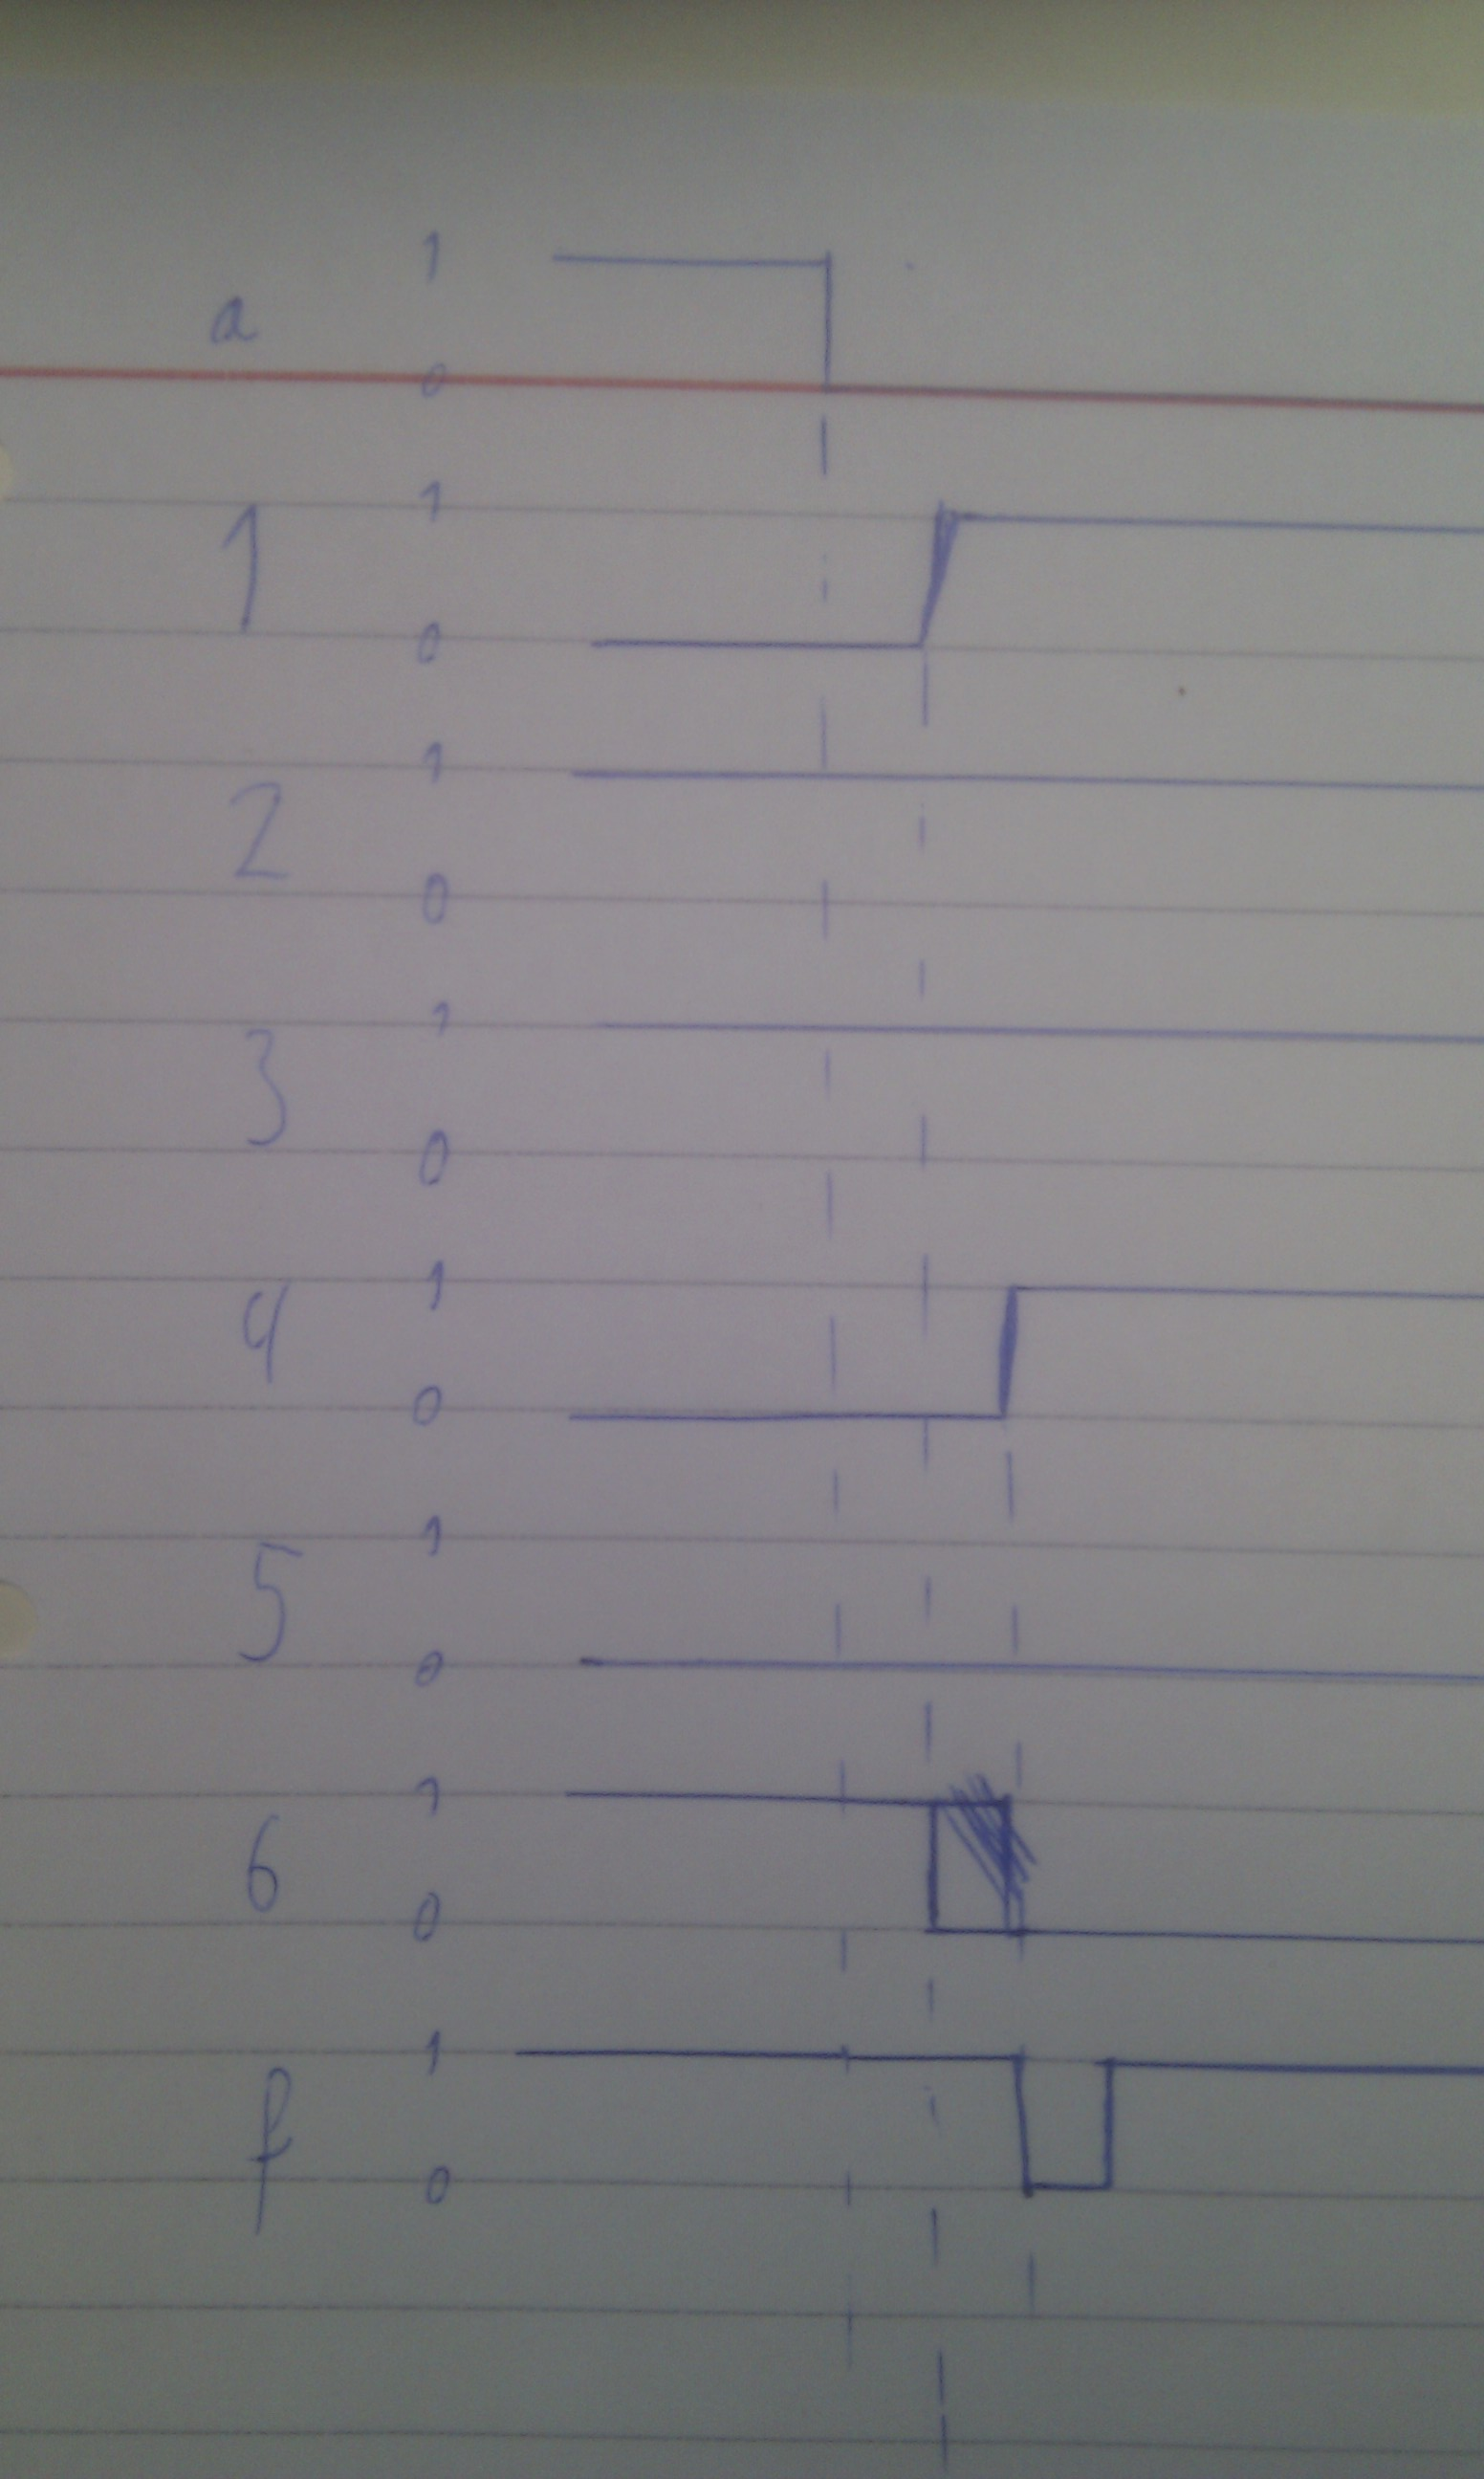
\includegraphics[width=200pt]{10_1_2}
\end{figure}
Es liegt ein statischer $1$-Hazard vor.
Die Schaltung implementiert die DNF von $f$.
Man könnte den Satz von Eichelberger ausnutzen und stattdessen beide Primimplikanten umsetzen: $\overline{b}\overline{c} + a\overline{c}$.

\section*{Aufgabe 10.2}

Ich werde keine Wahrheitstabelle benutzen, weil diese ziemlich groß wäre (16 Zeilen, 4 + 3 Spalten) und eine intuitive Implementierung durch XORs und Addierer möglich ist.
Wenn die Vermeidung von Hazards gefordert ist, wird die Wahrheitstabelle natürlich wieder Attraktiver, um z.B. den Satz von Eichelberger ausnutzen zu können.

\begin{figure}[H]
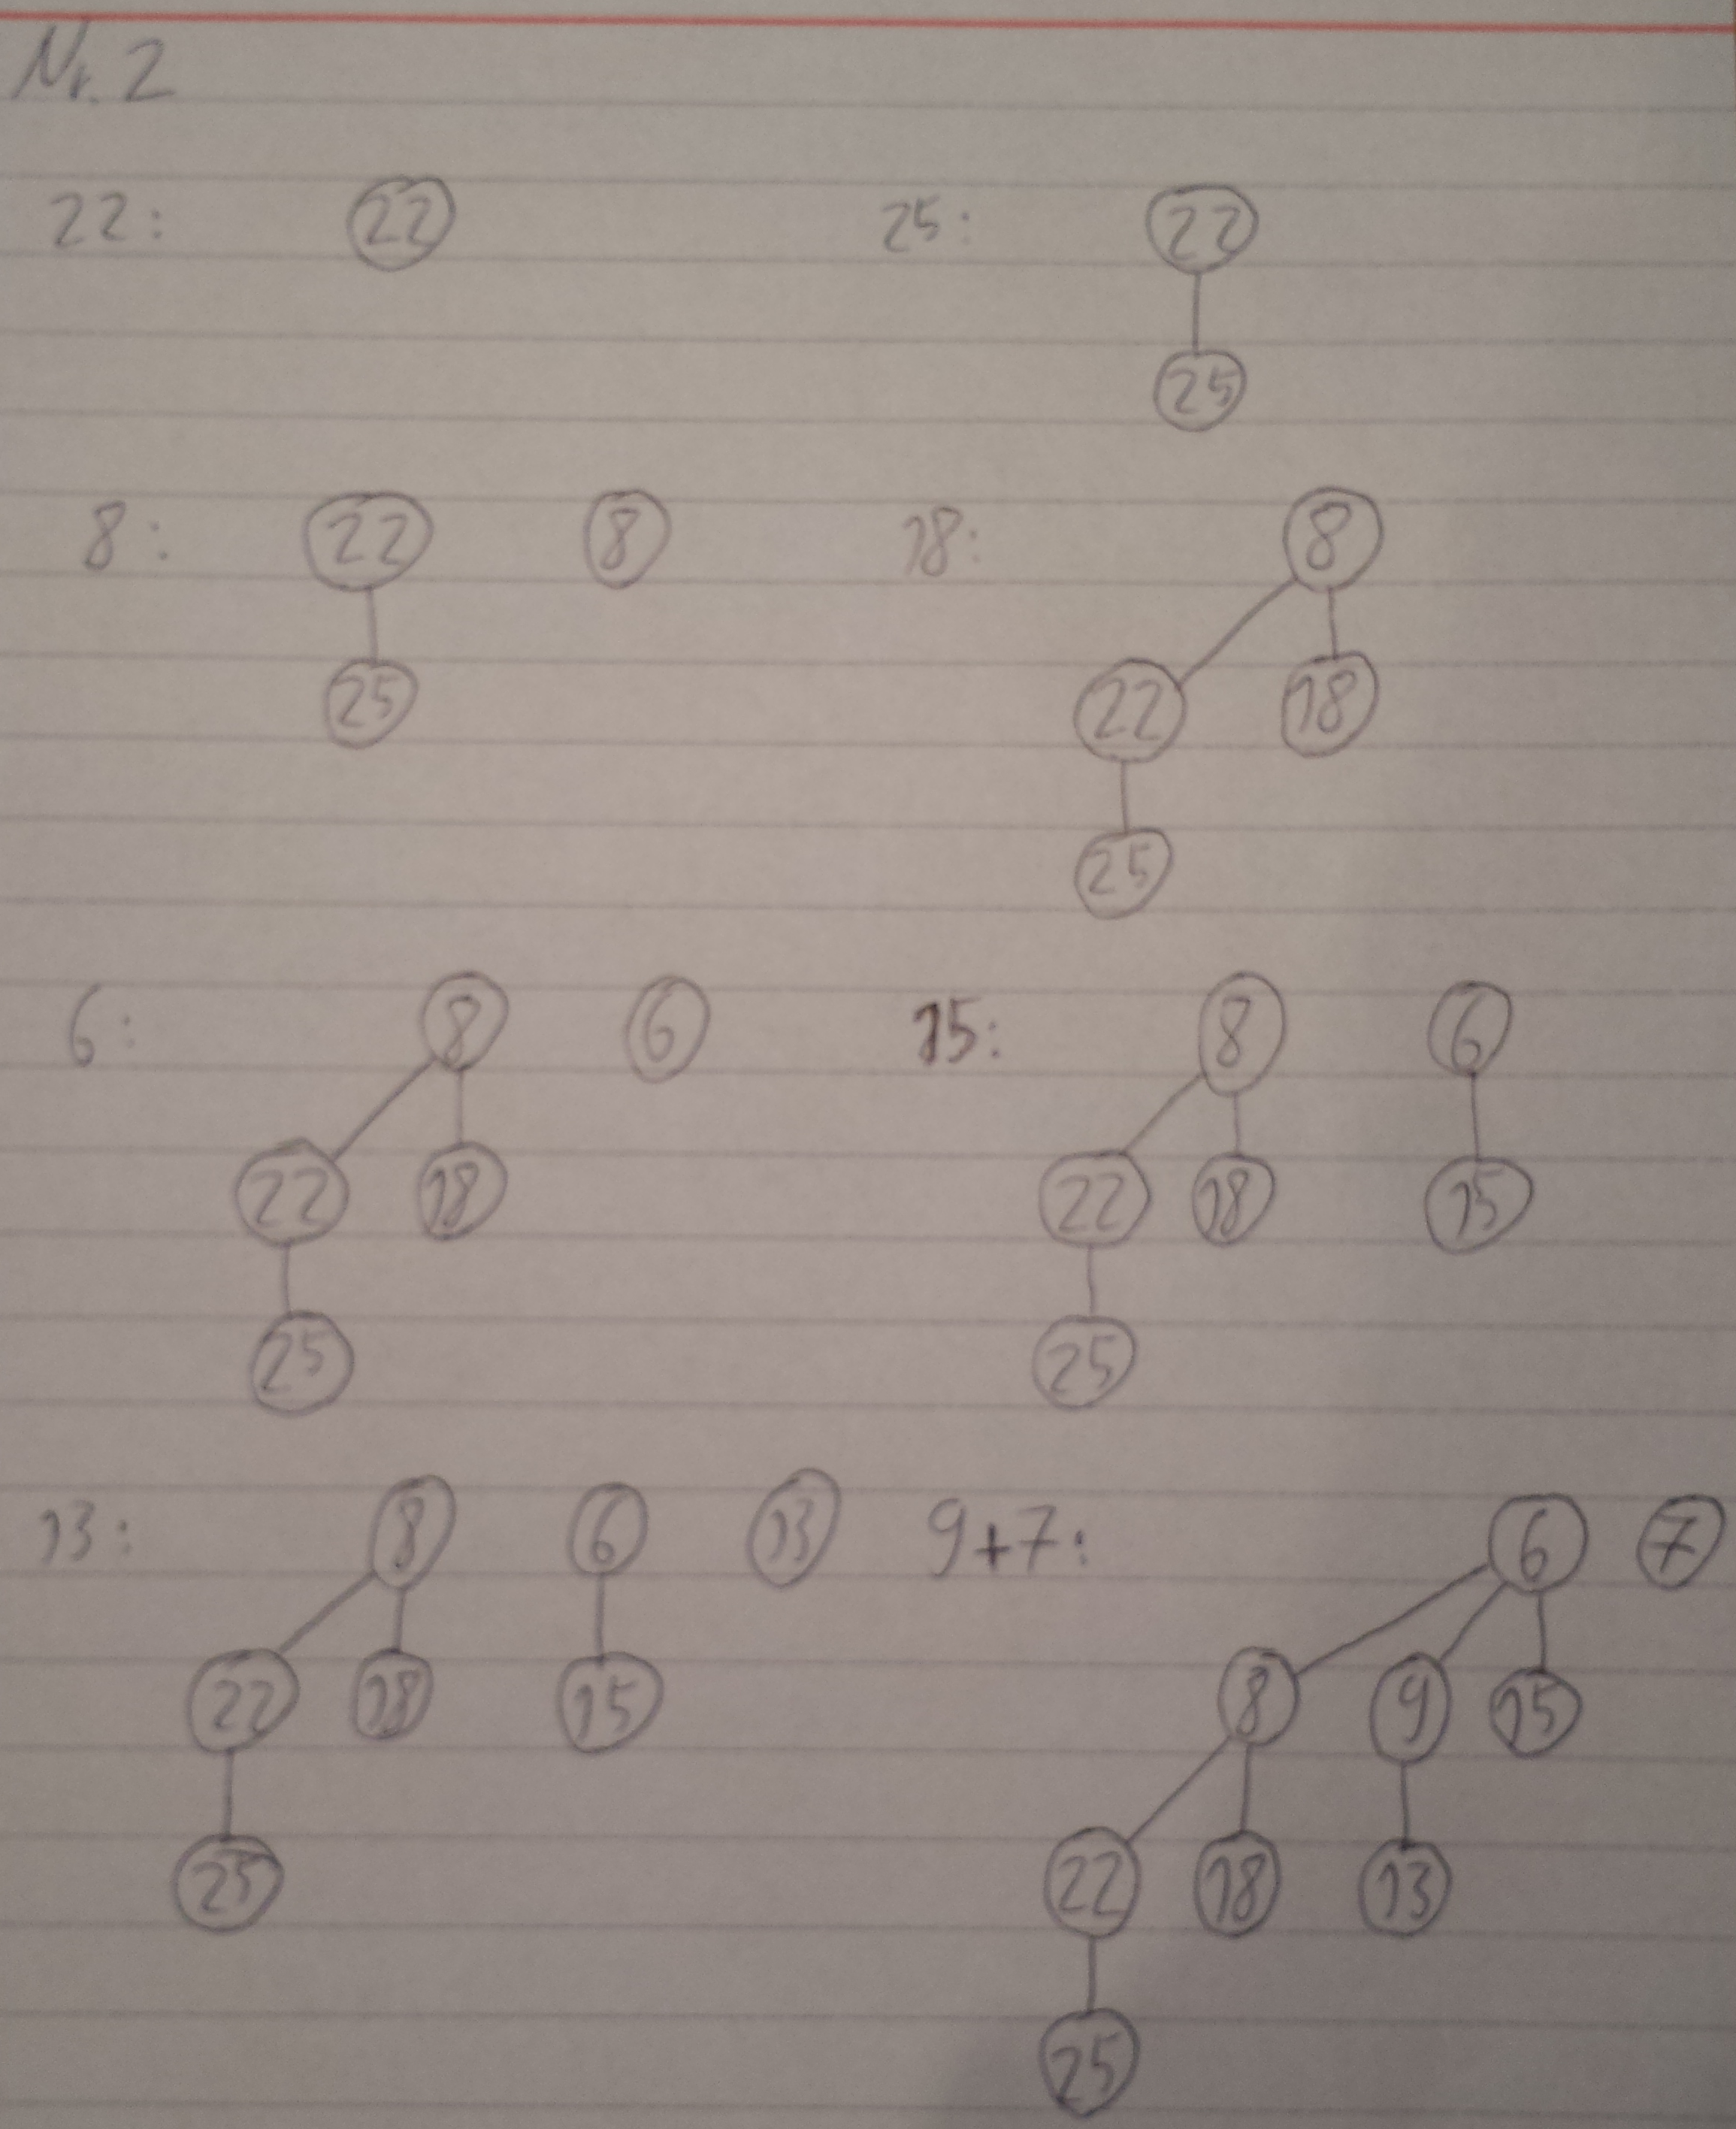
\includegraphics[width=300pt]{10_2}
\end{figure}

$a$ und $b$ sind die Eingaben und $c$ das Ergebnis.
$a_k$ ist das $2^k$-Bit der Variable.
Da es zwei Zahlen sind, können sie sich maximal an $4$ Stellen unterscheiden, was sich mit der 3-Bitzahl $c$ darstellen lässt.

Zuerst werden mit XOR-Gattern die unterschiedlichen Stellen berechnet.
Dann werden diese 4 1-Bitzahlen aufaddiert.
Jeweils zuerst 2 Stück zu zwei 2-Bitzahlen und dann diese beiden mittels eines Halb- und eines Volladdierers.

\section*{Aufgabe 10.3}

\begin{figure}[H]
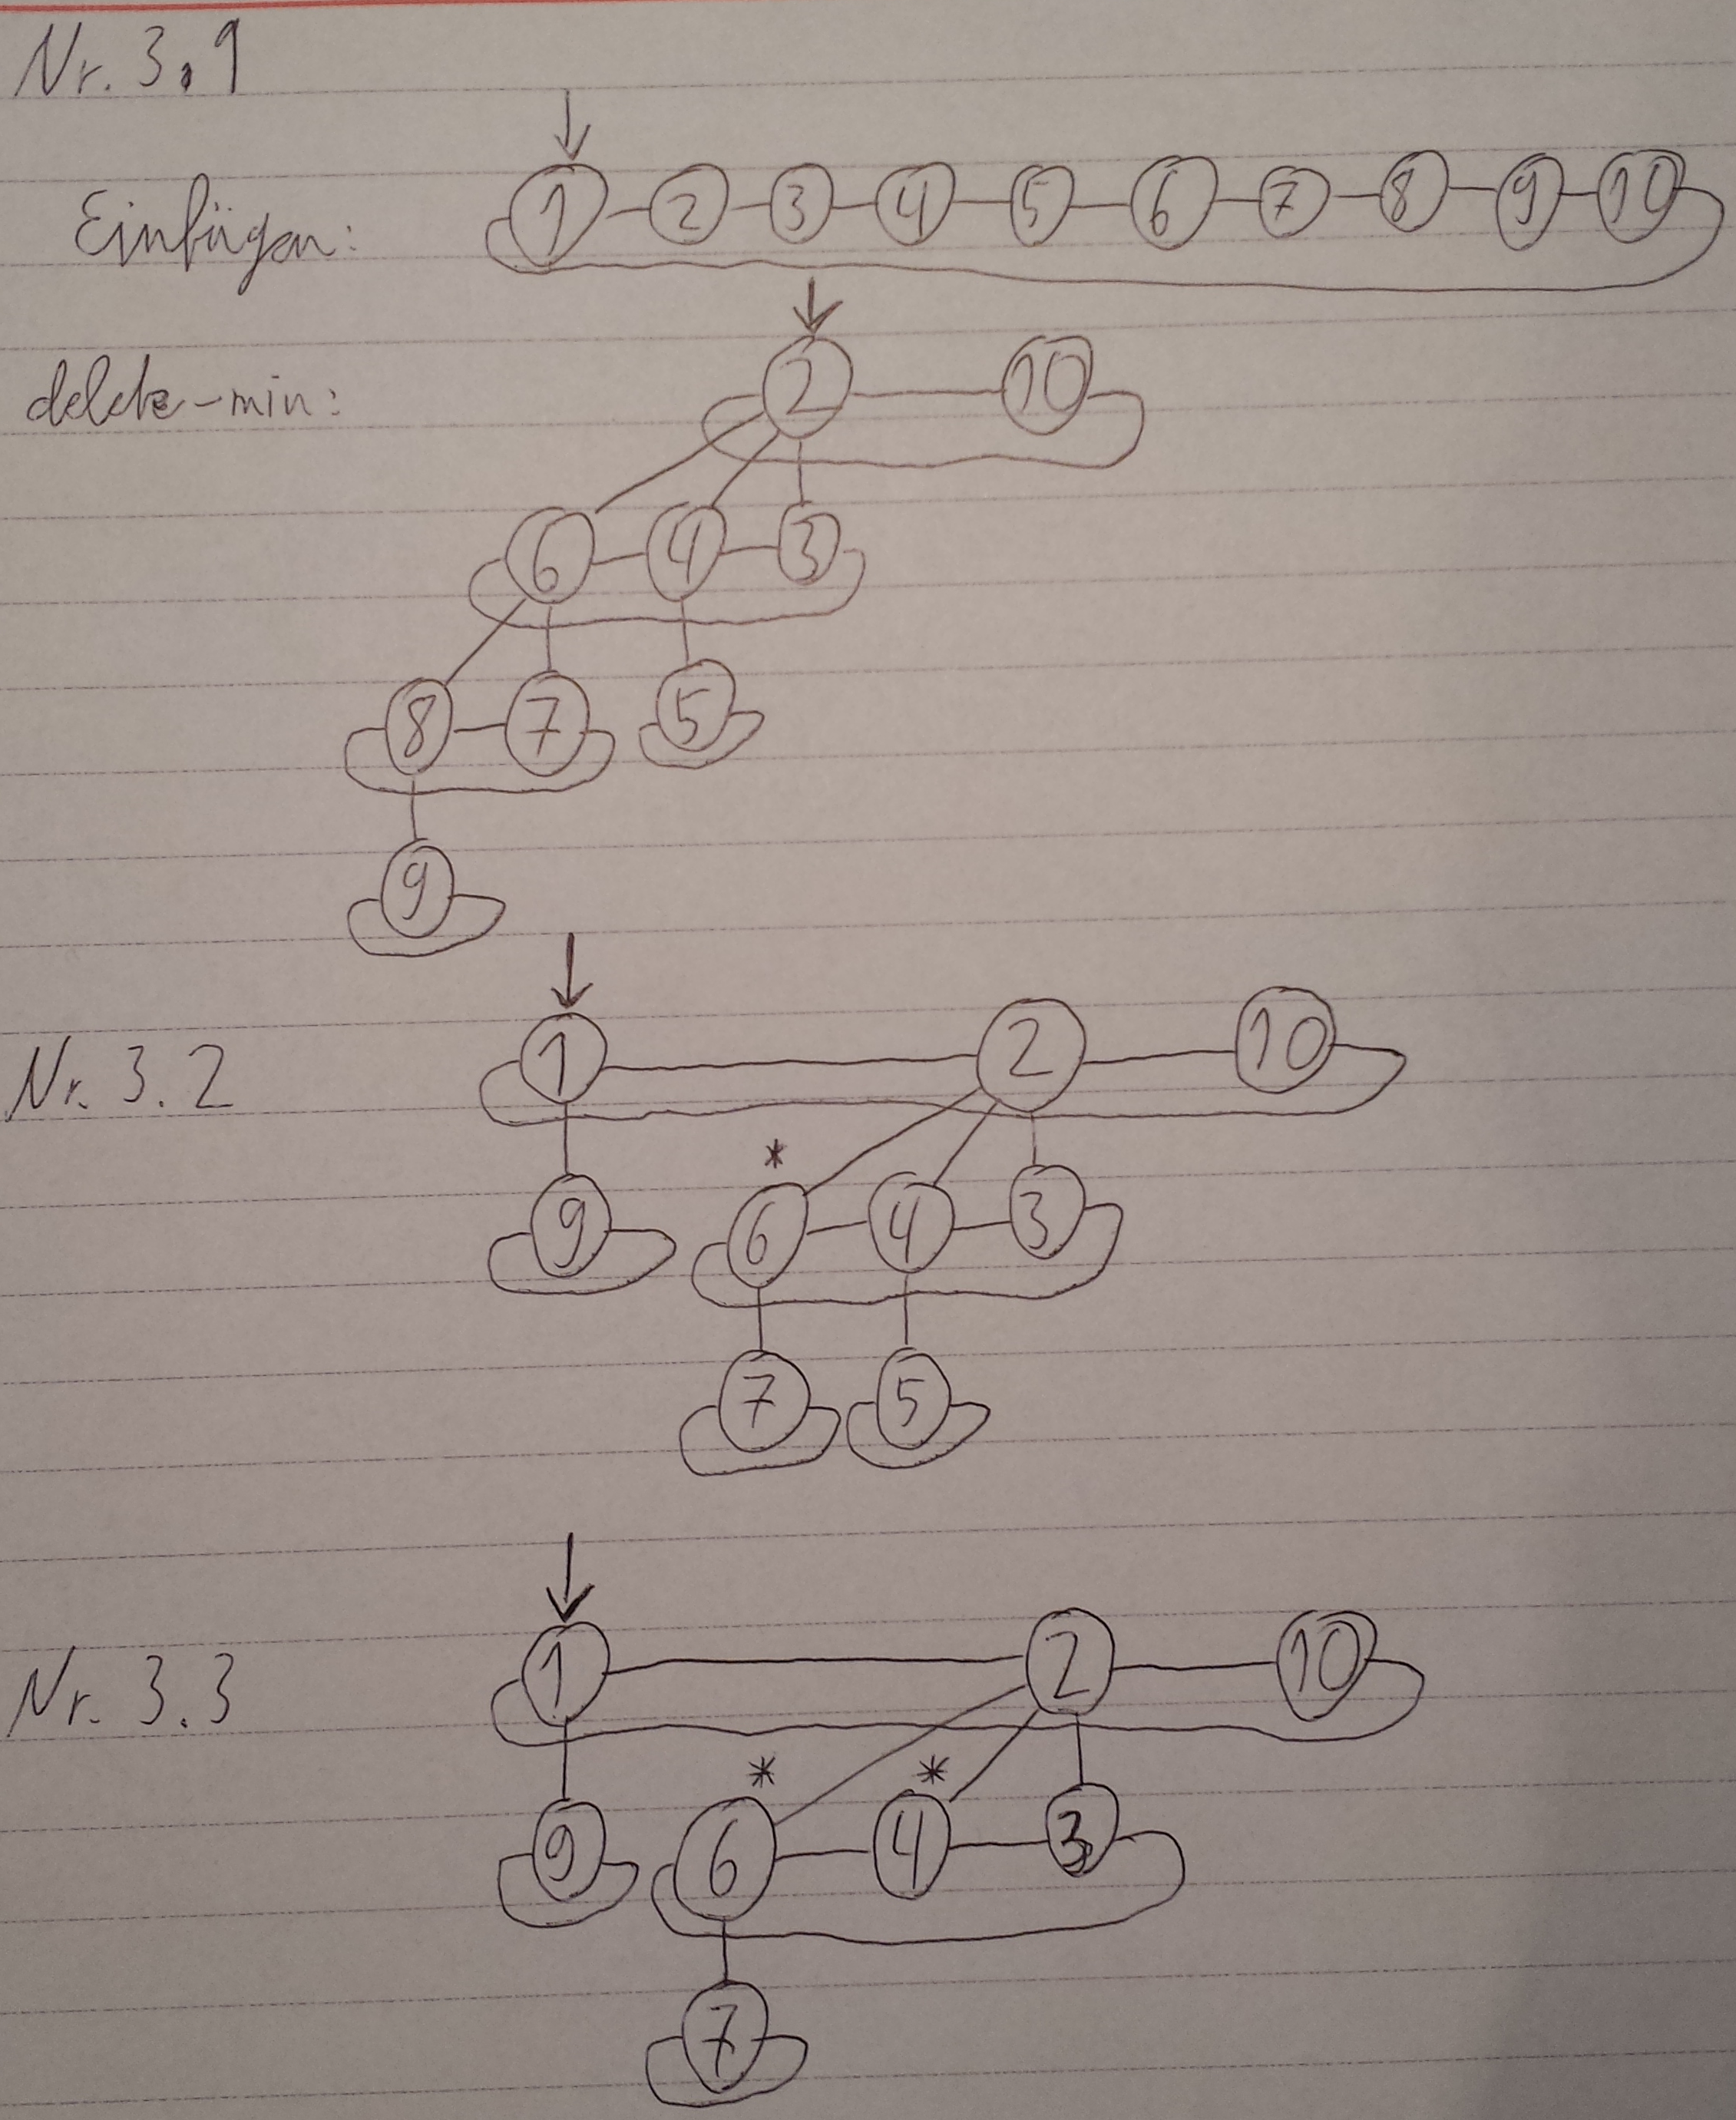
\includegraphics[width=500pt]{10_3}
\end{figure}

Zuerst werden die Paritäten berechnet und mit den gegebenen Paritäten verglichen.
Dann rechnet ein Decoder die Stellen der falschen Paritäten in die falsche Leitung um.
Diese wird dann invertiert, die anderen unverändert durchgereicht.

\section*{Aufgabe 10.4}

\begin{figure}[H]
\includegraphics[width=500pt]{10_4}
\end{figure}

\end{document}